\chapter{Introduction}
\label{Introduction}
The philosophy of human-centered design is to start a design process with a good understanding of the users and their needs. A common issue with developing products without involving the users in some way is that the products will be developed according to how the developers believe it should look and behave, and not how the users would expect it to. This will result in deficiencies for the users' interaction with the products, as they are likely to make mistakes and get confused. This is where good design becomes essential. If something unexpected happens, and the users are capable of easily fixing it, much satisfaction can arise for the users \parencite[][6-9]{PDF:DonNorman}. User experience design (UX) intends to provide the users with this satisfaction by designing products according to their needs, capabilities, and behaviour, which includes multiple aspects of branding, design, usability, and function \parencite{WEB:UXDesign}. This, however, haven't been fully integrated in the industry yet, as there still seems to be some misconception to what a human-centered design approach provides in development. This report will therefore start with an interpretation of the benefits of human-centered design in correlation with the terms UX and usability, before investigating different approaches for involving the users in the design process at a specific company.\\

\noindent
The danish tech company \textbf{TC Electronic (TC)} is the collaborating company for this purpose and has collaborated with students of Engineering Psychology on previous occasions. TC was originally formed in the early 1970's by Kim and John Rishøj in Aarhus, Denmark, and today they are worldwide known manufactorers of effect units for musicians. Besides effect units, they also produce other audio equipment such as amplifiers, sound and picture production systems, and broadcast systems \parencite{WEB:TCElectronic}. The collaboration was agreed upon through dialogue with TC themselves in shape of some mail correspondence before meeting with them at their headquarters and agreeing on a scope for the project. TC currently don't have a dedicated strategy for implementing methods for investigating UX and usability in their design process, but it is something they are interested in implementing in the development of future products.

\section{The benefits of human-centered design}
\label{UXbenefits}
The term \textit{user experience} was originally coined by Don Norman in 1993 while working at Apple. He defined it as everything that touches upon the user's experience with the product from first acquiring it to actually interacting with it and later evaluating this experience \parencite{WEB:DonNormanOnUX}. Numerous interpretations have since been formulated with $allaboutux.org$ containing a vast amount of these. Despite the differences in phrasing, what seems to be a common trait for these is that UX should be considered a broader term also covering other terms such as usability \parencite{WEB:UXDefinitions}. By investigating an ISO standard on human-centered design for interactive systems, this is emphazised, as UX is defined as \textit{a person's perceptions and responses resulting from the use and/or anticipated use of a product, system or service}. Three notes further elaborates how this includes all aspects of the person's emotions, beliefs, preferences, etc. \parencite[][3]{WEB:UXISO}. In the same ISO standard, usability is defined as \textit{the extend to which a product can be used for specified goals with effectiveness, efficiency and satisfaction in a specified context.} \parencite{WEB:UXISO}. Both these definitions support that UX should be considered the broader term, as usability is related to the functionality of a system, including the users' successes and failures during interaction, while UX also contains a hedonic aspect.\\

\noindent
Designing with a human-centered approach holds multiple benefits. \textcite{WEB:UXBenefits} describes these with regards to both the benefits for the users but also for the design process in general and the members of the design team. Firstly, if the developers in the company in question understand their users, they will then be able to understand the problems they may face by observing how they interact with a system. Secondly, sales increase when products satisfies their users. As it was mentioned in the introduction, a common issue is when products are developed solely from the developers' understanding of how it should look and behave. The developers then expect the users to have the same understanding, but since the users typically can't speak with the developers, the burden of communicating this understanding lies solely on the product itself including the documentations and manuals involved \parencite[][31]{PDF:DonNorman}. If it isn't clear to the users how they interact with the product, they won't have a satisfying experience with it. However, if the appropriate information is available to make the product understandable and usable, especially in situations when things go wrong, the users are then more likely to have a pleasent experience \parencite[][32]{PDF:DonNorman}. Finally, the development team itself can also benefit from a human-centered design approach. The better understanding of the users' needs, the design team have, the better their basis is for estimating the required amount of time and money for both development and subsequent maintenance of the product \parencite{WEB:UXBenefits}.\\

\noindent
Despite the outlined benefits of a human-centered approach to the design process, it is not yet fully integrated in the industry, and the reason for this lies in the difference of how the academic world develops methods for UX and usability testing, and how the industry utilizes these. Dennis Wixon stated in 2003 that \textit{"The literature evaluating usability methods is fundamentally flawed by its lack of relevance to applied usability work"} \parencite{WEB:WixonUXindustry}, this supports the concept of a gap between academia and industry. Several studies have since been made on this with \textcite{WEB:TinaOgLarsBo} being of interest. The purpose of this study was to investigate how 8 different companies changed how they worked within the fields of UX and usability over a period of 2 years. Interviews were held in 2013 and 2015 to uncover a positive development in the companies' understanding of UX and usability during these two years. Almost all of the companies had developed or were developing ways of implementing UX in their design process with examples such as low-fi prototyping, usability testing, workshops, personas, expert evaluations, etc. \parencite[][48]{WEB:TinaOgLarsBo}. In correlation with this, it is important to emphasize that almost all of these companies follows the agile \textit{Scrum} framework in their design process, which means that development is carried out as an iterative process in the form of sprints with the option of going back and making changes to the product in between these.\\

\noindent
More papers have recently been released on this topic and the challenges facing it. In a paper by \textcite{PDF:EvolutionofagileUXD}, the focus is on analyzing the evolution and current state of agile UX to provide a brief overview of theses challenges yet to be solved. It also takes its starting point in the increasing attention UX has gotten in the last 16 years, as designers and developers do understand the importance of each others work but don't know how to synchronize their daily operations in a meaningful way. As previously mentioned, the challenge lies in making UX relevant to the specific work in focus, but the challenge also lies in making everyone in the design team understand UX as a team discipline rather than a role in the team. As such, a more thorough understanding of UX and the agile framework is required to help both fields reach a shared understanding of  each other \parencite[][2]{PDF:EvolutionofagileUXD}. For \textcite{WEB:AgilityForUX} the focus is specifically on how UX and agility contribute to each other. The notion is that what helps a software developer to be agile may not help a UX consultant to be agile in the same way and vice versa. This is already well addressed as true, and the findings presented in the study further supports this notion. The study was conducted in an unspecified danish software company with \textit{Conboy's theory of agility} as research approach, which is elaborated on in the paper \parencite[][3]{WEB:AgilityForUX}. The study showed that the two practices contributed substantially different to agility for UX consultants and developers in correlation with different aspects of the design process. Finally, by consulting Nielsen Norman Group it is clear that despite the tendency of UX professionals perceiving Scrum meetings as barriers to productivity, they should still be involved in these meetings to stay engaged and aware of what's going on in the team \parencite{WEB:UXResponsibilitiesInScrum}. They propose that UX professionals take part in the scrum framework equivalently to any other member of the design team. This includes daily meetings addressing the questions \textit{what did you do yesterday?} \textit{what will you do today?} and \textit{what is in your way?}. This is considered important, as the UX professionals usually are working ahead of the development team. The UX professionals should furthermore engage in the work of the other members of the team, as they may be able to help resolve potential issues, they are facing.
%\newpage

\section{The Scrum framework}
\label{scrum}
As previously stated, much of the problem with employing a proper UX strategy in software development companies is due to UX not reconciling well with the agile scrum framework. The development teams of TC Electronic also employs this framework, and as such it seems fit to provide a proper description of it.

The scrum framework has gained popularity in the industry of developing software and hardware, as it has contributed to faster market times, greater flexibility, higher-quality products, and customer satisfaction \parencite[][40]{PDF:Scrum}. The overall concept is that the work is split into development iterations referred to as \textit{sprints}. These periods are typically of one month or less where a clear objective is set up and carried out by the \textit{Scrum team} which consists of the members of the development team. There are three different roles for the members, each expected to be self-organizing and cross-functional without being dependent on others outside the team \parencite[][41]{PDF:Scrum}.
%
\begin{itemize}
	\item \textbf{The Scrum Master} serves, much as the name indicates, as the leader of the Scrum Team. His primary objective is to make sure that the work to be done is understood and carried out by the Scrum Team.
	\item \textbf{The Product Owner} focuses on maximizing the work of the development team. He manages the list of requirements that the end product must meet, also known as the \textit{The Product Backlog}. This includes defining the backlog items and prioritizing them in order to optimize the value of the work done by the development team
	\item \textbf{The Development Team} consists of the remaining members of the Scrum Team, which typically is three professionals. Their goal is to execute the objectives established by The Product Owner and Scrum Master, and have them done by the end of sprint. 
\end{itemize}
%
The sprint starts with the initial planning by the members of the scrum team. During this phase they determine realistic goals for the sprint in correlation with what they want to achieve. The steps required to achieve their goals for the sprint are then determined from the backlog items as well through discussions with the product owner. When this is settled, the sprint starts. During the sprint, the team sets aside 15 minutes every day in order to synchronize activities and develop a plan for the next 24 hours. this is simply referred to as \textit{The Daily Scrum} \parencite[][41]{PDF:Scrum}. By the end of the sprint, the period is reviewed by the team in order to evaluate what has been achieved during the sprint, and what still needs to be done in order to complete the current sprint within the assigned time frame. Finally, a retrospective meeting inspects the sprint in order to discuss possible improvements for the next sprint to come. \autoref{fig:ScrumExplanation} provides a graphical elaboration of this process.
\newpage

\begin{figure}[H]
	\centering
	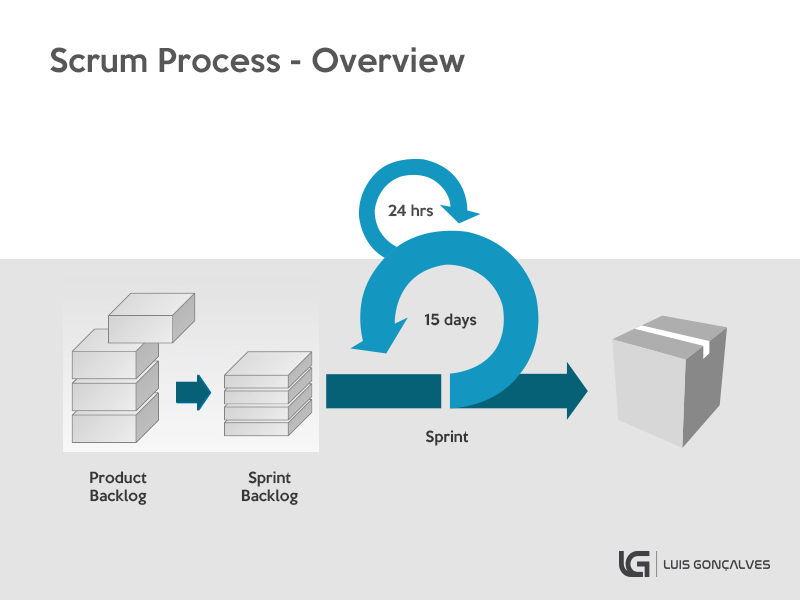
\includegraphics[width=\textwidth]{SCRUM.png}
	\caption{a graphical overview of the Scrum Process. \url{https://luis-goncalves.com/what-is-scrum-methodology/}}
	\label{fig:ScrumExplanation}
\end{figure}


\section{The TonePrint concept}
\label{TonePrintConceptDefined}
%Husk at 'Tweaking' ikke er et universelt ord, og der skal måske i stedet bruges 'editing' eller lignende.
An investigation of how TC can apply human-centered design approaches to their design process also requires focusing on a specific case in order to make it more relatable. Keeping it generic is expected to make it difficult to engage with for future design processes, and the choice was therefore made to use the plans for a future sharing platform for TonePrints as case in this project. Another term used for this platform is simply \textit{TonePrint community}, and for this to make more sense, it needs to be put into context with the general TonePrint concept. A description of this is therefore required, and this is done on the basis of three different papers released by TC themselves (\citeauthor{PDF:TonePrintAnalyse}; \citeyear{PDF:TonePrintAnalyse}; \citeyear{PDF:DesignforloebAfUserTonePrint}; \citeyear{PDF:BrugerWorkshopUserTonePrints}), including how they describe it on their own webpage \parencite{WEB:AboutTonePrints}. \\



\noindent
Effect pedals in general are well known units for guitarists and bassists alike, spanding multiple music genres. The pedal works by taking the input signal from the guitar and changing it to the tweaking by the users.

Depending on the effect type, and when playing, the user activates these changes by a single button on the pedal. An example of a simple guitar effect pedal is displayed on \autoref{fig:EffectPedalExample}, where the adjustable parameters on it consists of \textit{Dwell, Mix,} and \textit{Tone}. Each of these are accessed and tweaked with individual knobs on the unit, which gives the user a limited range of ways to change the sound. With this limitation as a motivation, TC created the TonePrint concept, enabling users to tweak the sound of effects beyond the parameters on the pedals. Using the TonePrint application, the users have a vast selection of custom presets with further parameters available for tweaking. These presets are what the term \textit{TonePrint} covers and they are either created in collaboration with professional musicians or by the common user. In order to distinguish these from each other, they are referred to as \textit{Artist TonePrints} and \textit{User TonePrints} respectively. After selecting one for the effect pedal in question, the user can make any desired tweaking or transfer it directly to the pedal with the option of altering it even more on the physical knobs \parencite{PDF:TonePrintAnalyse}. TC has collaborated with multiple guitarists and bassists, creating TonePrints for effect pedals used by the artists themselves. After the creators are satisfied with their TonePrints, they are uploaded to the TonePrint library in the application where any users of the same effect pedal can download the TonePrint and as such match the sound of their favourite artist. For User TonePrints the overall concept is the same. They differ in the fact that the creator isn't a famous guitarist, but the TonePrint is still made using the application and can be transferred directly to its effect pedal. However, when it comes to sharing these User TonePrint with friends and other aspiring guitarist, a platform for this purpose doesn't exist yet.


\begin{figure}[H]
	\centering
	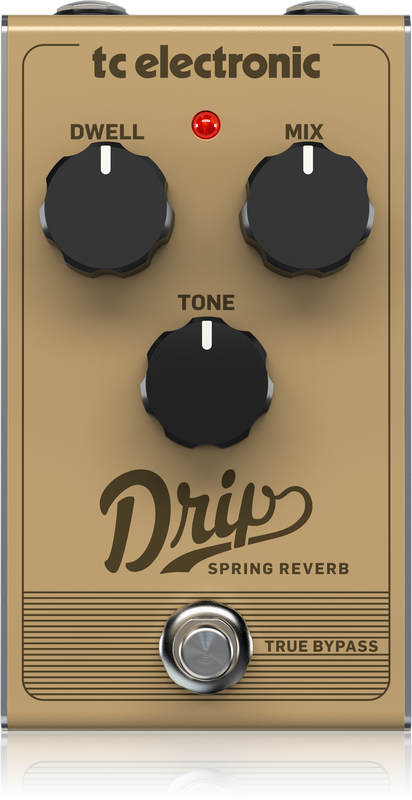
\includegraphics[width=.20\textwidth]{Graphics/EffectPedalExample}
	 \caption{This figure shows a Drip spring reverb effect pedal by TC Electronic \url{https://www.tcelectronic.com/Categories/Tcelectronic/Guitar/Stompboxes/DRIP-SPRING-REVERB/p/P0CQ2\#googtrans(en|en)}.}
    \label{fig:EffectPedalExample}
\end{figure}


\subsection{The TonePrint Software}
\label{TonePrintSoftware}
\fxnote{Overvej om der skal være et billede af editoren of en kort forklaring af stepne til at lave et TonePrint}As previously stated, the exploring of TonePrints start with the TonePrint application available for smartphones and tablets. However, the software is also available for PC and MAC, and the reason for this distinction lies in the difference of how a TonePrint is transferred to its respective pedal. For PC and MAC the user is required to use a cable from the computer to the pedal, but through the tablet and smartphone application, the user also have the option of beaming it directly to the pedal. whatever the platform, however, when opening the software the user is introduced to a list selection of different effect pedals, each holding a vast number of TonePrints created by famous guitarists. After selecting an effect pedal from this list, the user is then presented a new list selection of the many guitarist who have created TonePrints for this pedal. When selecting one of the guitarists, and depending on whether the guitarist have created more TonePrints for the same pedal, the user is then presented a bigger view of this specific TonePrint with a description of it and its creator. An example of this is displayed on \autoref{fig:TonePrintAppExample}. Depending on the users' motivation when opening the application first time, they can also choose to browse by artist instead of pedal, if their starting point is to find out what it takes to sound like their favourite artist.
%
\begin{figure}[H]
	\centering
	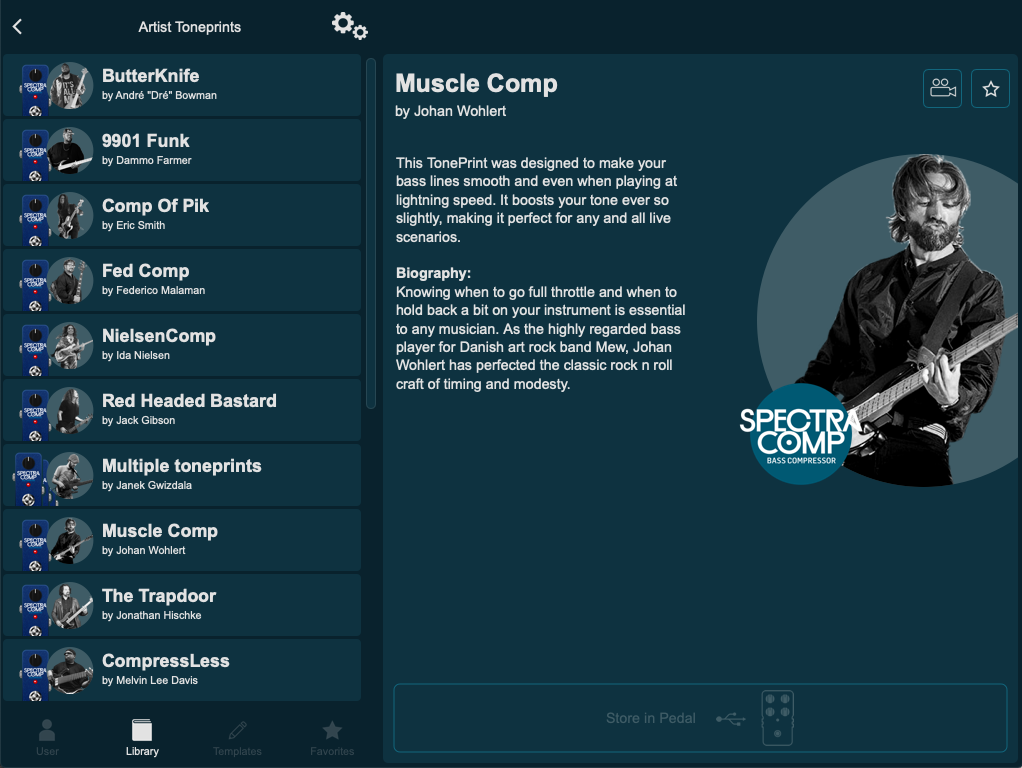
\includegraphics[width=0.75\textwidth]{TonePrintAppExample}
	\caption{The view in the TonePrint application after selecting an effect pedal and a TonePrint. This example displays a TonePrint created by Johan Wohlert of the danish rock band \textit{Mew}.}
	\label{fig:TonePrintAppExample}
\end{figure}

\newpage
%
\section{Research question}
\label{ResearchQuestion}
%
The scope of this project is elaborated though the sections of  \autoref{Introduction} which focus on different aspects that will work as a base of this project. As mentioned is the scope helping TC towards a more user centered design process and doing this in the context of the design process of the future product TonePrint community. This leads to the establishment of a research question that this project will work towards answering. The research question is as following:

\begin{quote}
	\textbf{\textit{How may methods of user centered design be applied for the design process of the TonePrint Community?}}
\end{quote}
